
%% bare_jrnl.tex
%% V1.3
%% 2007/01/11
%% by Michael Shell
%% see http://www.michaelshell.org/
%% for current contact information.
%%
%% This is a skeleton file demonstrating the use of IEEEtran.cls
%% (requires IEEEtran.cls version 1.7 or later) with an IEEE journal paper.
%%
%% Support sites:
%% http://www.michaelshell.org/tex/ieeetran/
%% http://www.ctan.org/tex-archive/macros/latex/contrib/IEEEtran/
%% and
%% http://www.ieee.org/



% *** Authors should verify (and, if needed, correct) their LaTeX system  ***
% *** with the testflow diagnostic prior to trusting their LaTeX platform ***
% *** with production work. IEEE's font choices can trigger bugs that do  ***
% *** not appear when using other class files.                            ***
% The testflow support page is at:
% http://www.michaelshell.org/tex/testflow/


%%*************************************************************************
%% Legal Notice:
%% This code is offered as-is without any warranty either expressed or
%% implied; without even the implied warranty of MERCHANTABILITY or
%% FITNESS FOR A PARTICULAR PURPOSE! 
%% User assumes all risk.
%% In no event shall IEEE or any contributor to this code be liable for
%% any damages or losses, including, but not limited to, incidental,
%% consequential, or any other damages, resulting from the use or misuse
%% of any information contained here.
%%
%% All comments are the opinions of their respective authors and are not
%% necessarily endorsed by the IEEE.
%%
%% This work is distributed under the LaTeX Project Public License (LPPL)
%% ( http://www.latex-project.org/ ) version 1.3, and may be freely used,
%% distributed and modified. A copy of the LPPL, version 1.3, is included
%% in the base LaTeX documentation of all distributions of LaTeX released
%% 2003/12/01 or later.
%% Retain all contribution notices and credits.
%% ** Modified files should be clearly indicated as such, including  **
%% ** renaming them and changing author support contact information. **
%%
%% File list of work: IEEEtran.cls, IEEEtran_HOWTO.pdf, bare_adv.tex,
%%                    bare_conf.tex, bare_jrnl.tex, bare_jrnl_compsoc.tex
%%*************************************************************************

% Note that the a4paper option is mainly intended so that authors in
% countries using A4 can easily print to A4 and see how their papers will
% look in print - the typesetting of the document will not typically be
% affected with changes in paper size (but the bottom and side margins will).
% Use the testflow package mentioned above to verify correct handling of
% both paper sizes by the user's LaTeX system.
%
% Also note that the "draftcls" or "draftclsnofoot", not "draft", option
% should be used if it is desired that the figures are to be displayed in
% draft mode.
%
\documentclass[journal]{IEEEtran}
\usepackage{blindtext}
\usepackage{graphicx}
\usepackage{float}
\usepackage{csquotes}
% Some very useful LaTeX packages include:
% (uncomment the ones you want to load)


% *** MISC UTILITY PACKAGES ***
%
%\usepackage{ifpdf}
% Heiko Oberdiek's ifpdf.sty is very useful if you need conditional
% compilation based on whether the output is pdf or dvi.
% usage:
% \ifpdf
%   % pdf code
% \else
%   % dvi code
% \fi
% The latest version of ifpdf.sty can be obtained from:
% http://www.ctan.org/tex-archive/macros/latex/contrib/oberdiek/
% Also, note that IEEEtran.cls V1.7 and later provides a builtin
% \ifCLASSINFOpdf conditional that works the same way.
% When switching from latex to pdflatex and vice-versa, the compiler may
% have to be run twice to clear warning/error messages.






% *** CITATION PACKAGES ***
%
%\usepackage{cite}
% cite.sty was written by Donald Arseneau
% V1.6 and later of IEEEtran pre-defines the format of the cite.sty package
% \cite{} output to follow that of IEEE. Loading the cite package will
% result in citation numbers being automatically sorted and properly
% "compressed/ranged". e.g., [1], [9], [2], [7], [5], [6] without using
% cite.sty will become [1], [2], [5]--[7], [9] using cite.sty. cite.sty's
% \cite will automatically add leading space, if needed. Use cite.sty's
% noadjust option (cite.sty V3.8 and later) if you want to turn this off.
% cite.sty is already installed on most LaTeX systems. Be sure and use
% version 4.0 (2003-05-27) and later if using hyperref.sty. cite.sty does
% not currently provide for hyperlinked citations.
% The latest version can be obtained at:
% http://www.ctan.org/tex-archive/macros/latex/contrib/cite/
% The documentation is contained in the cite.sty file itself.






% *** GRAPHICS RELATED PACKAGES ***
%
\ifCLASSINFOpdf
  % \usepackage[pdftex]{graphicx}
  % declare the path(s) where your graphic files are
  % \graphicspath{{../pdf/}{../jpeg/}}
  % and their extensions so you won't have to specify these with
  % every instance of \includegraphics
  % \DeclareGraphicsExtensions{.pdf,.jpeg,.png}
\else
  % or other class option (dvipsone, dvipdf, if not using dvips). graphicx
  % will default to the driver specified in the system graphics.cfg if no
  % driver is specified.
  % \usepackage[dvips]{graphicx}
  % declare the path(s) where your graphic files are
  % \graphicspath{{../eps/}}
  % and their extensions so you won't have to specify these with
  % every instance of \includegraphics
  % \DeclareGraphicsExtensions{.eps}
\fi
% graphicx was written by David Carlisle and Sebastian Rahtz. It is
% required if you want graphics, photos, etc. graphicx.sty is already
% installed on most LaTeX systems. The latest version and documentation can
% be obtained at: 
% http://www.ctan.org/tex-archive/macros/latex/required/graphics/
% Another good source of documentation is "Using Imported Graphics in
% LaTeX2e" by Keith Reckdahl which can be found as epslatex.ps or
% epslatex.pdf at: http://www.ctan.org/tex-archive/info/
%
% latex, and pdflatex in dvi mode, support graphics in encapsulated
% postscript (.eps) format. pdflatex in pdf mode supports graphics
% in .pdf, .jpeg, .png and .mps (metapost) formats. Users should ensure
% that all non-photo figures use a vector format (.eps, .pdf, .mps) and
% not a bitmapped formats (.jpeg, .png). IEEE frowns on bitmapped formats
% which can result in "jaggedy"/blurry rendering of lines and letters as
% well as large increases in file sizes.
%
% You can find documentation about the pdfTeX application at:
% http://www.tug.org/applications/pdftex


%URL package for url links in the bibliography
\usepackage{url}


% *** MATH PACKAGES ***
%
\usepackage[cmex10]{amsmath}
\usepackage{bm}
% A popular package from the American Mathematical Society that provides
% many useful and powerful commands for dealing with mathematics. If using
% it, be sure to load this package with the cmex10 option to ensure that
% only type 1 fonts will utilized at all point sizes. Without this option,
% it is possible that some math symbols, particularly those within
% footnotes, will be rendered in bitmap form which will result in a
% document that can not be IEEE Xplore compliant!
%
% Also, note that the amsmath package sets \interdisplaylinepenalty to 10000
% thus preventing page breaks from occurring within multiline equations. Use:
\interdisplaylinepenalty=2500
% after loading amsmath to restore such page breaks as IEEEtran.cls normally
% does. amsmath.sty is already installed on most LaTeX systems. The latest
% version and documentation can be obtained at:
% http://www.ctan.org/tex-archive/macros/latex/required/amslatex/math/





% *** SPECIALIZED LIST PACKAGES ***
%
%\usepackage{algorithmic}
% algorithmic.sty was written by Peter Williams and Rogerio Brito.
% This package provides an algorithmic environment fo describing algorithms.
% You can use the algorithmic environment in-text or within a figure
% environment to provide for a floating algorithm. Do NOT use the algorithm
% floating environment provided by algorithm.sty (by the same authors) or
% algorithm2e.sty (by Christophe Fiorio) as IEEE does not use dedicated
% algorithm float types and packages that provide these will not provide
% correct IEEE style captions. The latest version and documentation of
% algorithmic.sty can be obtained at:
% http://www.ctan.org/tex-archive/macros/latex/contrib/algorithms/
% There is also a support site at:
% http://algorithms.berlios.de/index.html
% Also of interest may be the (relatively newer and more customizable)
% algorithmicx.sty package by Szasz Janos:
% http://www.ctan.org/tex-archive/macros/latex/contrib/algorithmicx/




% *** ALIGNMENT PACKAGES ***
%
%\usepackage{array}
% Frank Mittelbach's and David Carlisle's array.sty patches and improves
% the standard LaTeX2e array and tabular environments to provide better
% appearance and additional user controls. As the default LaTeX2e table
% generation code is lacking to the point of almost being broken with
% respect to the quality of the end results, all users are strongly
% advised to use an enhanced (at the very least that provided by array.sty)
% set of table tools. array.sty is already installed on most systems. The
% latest version and documentation can be obtained at:
% http://www.ctan.org/tex-archive/macros/latex/required/tools/


%\usepackage{mdwmath}
%\usepackage{mdwtab}
% Also highly recommended is Mark Wooding's extremely powerful MDW tools,
% especially mdwmath.sty and mdwtab.sty which are used to format equations
% and tables, respectively. The MDWtools set is already installed on most
% LaTeX systems. The lastest version and documentation is available at:
% http://www.ctan.org/tex-archive/macros/latex/contrib/mdwtools/


% IEEEtran contains the IEEEeqnarray family of commands that can be used to
% generate multiline equations as well as matrices, tables, etc., of high
% quality.


%\usepackage{eqparbox}
% Also of notable interest is Scott Pakin's eqparbox package for creating
% (automatically sized) equal width boxes - aka "natural width parboxes".
% Available at:
% http://www.ctan.org/tex-archive/macros/latex/contrib/eqparbox/





% *** SUBFIGURE PACKAGES ***
%\usepackage[tight,footnotesize]{subfigure}
% subfigure.sty was written by Steven Douglas Cochran. This package makes it
% easy to put subfigures in your figures. e.g., "Figure 1a and 1b". For IEEE
% work, it is a good idea to load it with the tight package option to reduce
% the amount of white space around the subfigures. subfigure.sty is already
% installed on most LaTeX systems. The latest version and documentation can
% be obtained at:
% http://www.ctan.org/tex-archive/obsolete/macros/latex/contrib/subfigure/
% subfigure.sty has been superceeded by subfig.sty.



%\usepackage[caption=false]{caption}
%\usepackage[font=footnotesize]{subfig}
% subfig.sty, also written by Steven Douglas Cochran, is the modern
% replacement for subfigure.sty. However, subfig.sty requires and
% automatically loads Axel Sommerfeldt's caption.sty which will override
% IEEEtran.cls handling of captions and this will result in nonIEEE style
% figure/table captions. To prevent this problem, be sure and preload
% caption.sty with its "caption=false" package option. This is will preserve
% IEEEtran.cls handing of captions. Version 1.3 (2005/06/28) and later 
% (recommended due to many improvements over 1.2) of subfig.sty supports
% the caption=false option directly:
%\usepackage[caption=false,font=footnotesize]{subfig}
%
% The latest version and documentation can be obtained at:
% http://www.ctan.org/tex-archive/macros/latex/contrib/subfig/
% The latest version and documentation of caption.sty can be obtained at:
% http://www.ctan.org/tex-archive/macros/latex/contrib/caption/




% *** FLOAT PACKAGES ***
%
%\usepackage{fixltx2e}
% fixltx2e, the successor to the earlier fix2col.sty, was written by
% Frank Mittelbach and David Carlisle. This package corrects a few problems
% in the LaTeX2e kernel, the most notable of which is that in current
% LaTeX2e releases, the ordering of single and double column floats is not
% guaranteed to be preserved. Thus, an unpatched LaTeX2e can allow a
% single column figure to be placed prior to an earlier double column
% figure. The latest version and documentation can be found at:
% http://www.ctan.org/tex-archive/macros/latex/base/



%\usepackage{stfloats}
% stfloats.sty was written by Sigitas Tolusis. This package gives LaTeX2e
% the ability to do double column floats at the bottom of the page as well
% as the top. (e.g., "\begin{figure*}[!b]" is not normally possible in
% LaTeX2e). It also provides a command:
%\fnbelowfloat
% to enable the placement of footnotes below bottom floats (the standard
% LaTeX2e kernel puts them above bottom floats). This is an invasive package
% which rewrites many portions of the LaTeX2e float routines. It may not work
% with other packages that modify the LaTeX2e float routines. The latest
% version and documentation can be obtained at:
% http://www.ctan.org/tex-archive/macros/latex/contrib/sttools/
% Documentation is contained in the stfloats.sty comments as well as in the
% presfull.pdf file. Do not use the stfloats baselinefloat ability as IEEE
% does not allow \baselineskip to stretch. Authors submitting work to the
% IEEE should note that IEEE rarely uses double column equations and
% that authors should try to avoid such use. Do not be tempted to use the
% cuted.sty or midfloat.sty packages (also by Sigitas Tolusis) as IEEE does
% not format its papers in such ways.


%\ifCLASSOPTIONcaptionsoff
%  \usepackage[nomarkers]{endfloat}
% \let\MYoriglatexcaption\caption
% \renewcommand{\caption}[2][\relax]{\MYoriglatexcaption[#2]{#2}}
%\fi
% endfloat.sty was written by James Darrell McCauley and Jeff Goldberg.
% This package may be useful when used in conjunction with IEEEtran.cls'
% captionsoff option. Some IEEE journals/societies require that submissions
% have lists of figures/tables at the end of the paper and that
% figures/tables without any captions are placed on a page by themselves at
% the end of the document. If needed, the draftcls IEEEtran class option or
% \CLASSINPUTbaselinestretch interface can be used to increase the line
% spacing as well. Be sure and use the nomarkers option of endfloat to
% prevent endfloat from "marking" where the figures would have been placed
% in the text. The two hack lines of code above are a slight modification of
% that suggested by in the endfloat docs (section 8.3.1) to ensure that
% the full captions always appear in the list of figures/tables - even if
% the user used the short optional argument of \caption[]{}.
% IEEE papers do not typically make use of \caption[]'s optional argument,
% so this should not be an issue. A similar trick can be used to disable
% captions of packages such as subfig.sty that lack options to turn off
% the subcaptions:
% For subfig.sty:
% \let\MYorigsubfloat\subfloat
% \renewcommand{\subfloat}[2][\relax]{\MYorigsubfloat[]{#2}}
% For subfigure.sty:
% \let\MYorigsubfigure\subfigure
% \renewcommand{\subfigure}[2][\relax]{\MYorigsubfigure[]{#2}}
% However, the above trick will not work if both optional arguments of
% the \subfloat/subfig command are used. Furthermore, there needs to be a
% description of each subfigure *somewhere* and endfloat does not add
% subfigure captions to its list of figures. Thus, the best approach is to
% avoid the use of subfigure captions (many IEEE journals avoid them anyway)
% and instead reference/explain all the subfigures within the main caption.
% The latest version of endfloat.sty and its documentation can obtained at:
% http://www.ctan.org/tex-archive/macros/latex/contrib/endfloat/
%
% The IEEEtran \ifCLASSOPTIONcaptionsoff conditional can also be used
% later in the document, say, to conditionally put the References on a 
% page by themselves.





% *** PDF, URL AND HYPERLINK PACKAGES ***
%
%\usepackage{url}
% url.sty was written by Donald Arseneau. It provides better support for
% handling and breaking URLs. url.sty is already installed on most LaTeX
% systems. The latest version can be obtained at:
% http://www.ctan.org/tex-archive/macros/latex/contrib/misc/
% Read the url.sty source comments for usage information. Basically,
% \url{my_url_here}.





% *** Do not adjust lengths that control margins, column widths, etc. ***
% *** Do not use packages that alter fonts (such as pslatex).         ***
% There should be no need to do such things with IEEEtran.cls V1.6 and later.
% (Unless specifically asked to do so by the journal or conference you plan
% to submit to, of course. )


% correct bad hyphenation here
\hyphenation{op-tical net-works semi-conduc-tor}


\begin{document}
%
% paper title
% can use linebreaks \\ within to get better formatting as desired
\title{Solving Travelling Salesman Problems with Genetic Algorithms}
%
%
% author names and IEEE memberships
% note positions of commas and nonbreaking spaces ( ~ ) LaTeX will not break
% a structure at a ~ so this keeps an author's name from being broken across
% two lines.
% use \thanks{} to gain access to the first footnote area
% a separate \thanks must be used for each paragraph as LaTeX2e's \thanks
% was not built to handle multiple paragraphs
%

\author{Samuel Jackson, University of Aberystwyth}

% note the % following the last \IEEEmembership and also \thanks - 
% these prevent an unwanted space from occurring between the last author name
% and the end of the author line. i.e., if you had this:
% 
% \author{....lastname \thanks{...} \thanks{...} }
%                     ^------------^------------^----Do not want these spaces!
%
% a space would be appended to the last name and could cause every name on that
% line to be shifted left slightly. This is one of those "LaTeX things". For
% instance, "\textbf{A} \textbf{B}" will typeset as "A B" not "AB". To get
% "AB" then you have to do: "\textbf{A}\textbf{B}"
% \thanks is no different in this regard, so shield the last } of each \thanks
% that ends a line with a % and do not let a space in before the next \thanks.
% Spaces after \IEEEmembership other than the last one are OK (and needed) as
% you are supposed to have spaces between the names. For what it is worth,
% this is a minor point as most people would not even notice if the said evil
% space somehow managed to creep in.



% The paper headers
%\markboth{Journal of \LaTeX\ Class Files,~Vol.~6, No.~1, January~2007}%
%{Shell \MakeLowercase{\textit{et al.}}: Bare Demo of IEEEtran.cls for Journals}
% The only time the second header will appear is for the odd numbered pages
% after the title page when using the twoside option.
% 
% *** Note that you probably will NOT want to include the author's ***
% *** name in the headers of peer review papers.                   ***
% You can use \ifCLASSOPTIONpeerreview for conditional compilation here if
% you desire.




% If you want to put a publisher's ID mark on the page you can do it like
% this:
%\IEEEpubid{0000--0000/00\$00.00~\copyright~2007 IEEE}
% Remember, if you use this you must call \IEEEpubidadjcol in the second
% column for its text to clear the IEEEpubid mark.



% use for special paper notices
%\IEEEspecialpapernotice{(Invited Paper)}




% make the title area
\maketitle


%\begin{abstract}
%\boldmath
%\blindtext[1]
%\end{abstract}
% IEEEtran.cls defaults to using nonbold math in the Abstract.
% This preserves the distinction between vectors and scalars. However,
% if the journal you are submitting to favors bold math in the abstract,
% then you can use LaTeX's standard command \boldmath at the very start
% of the abstract to achieve this. Many IEEE journals frown on math
% in the abstract anyway.

% Note that keywords are not normally used for peerreview papers.
%\begin{IEEEkeywords}
%IEEEtran, journal, \LaTeX, paper, template.
%\end{IEEEkeywords}






% For peer review papers, you can put extra information on the cover
% page as needed:
% \ifCLASSOPTIONpeerreview
% \begin{center} \bfseries EDICS Category: 3-BBND \end{center}
% \fi
%
% For peerreview papers, this IEEEtran command inserts a page break and
% creates the second title. It will be ignored for other modes.
\IEEEpeerreviewmaketitle



\section{Introduction}

\noindent 
A genetic algorithm (GA) is a search and optimisation method frequently used to find approximate solutions in challenging problem domains. Genetic algorithms are inspired by the biological concept of natural selection. This places genetic algorithms under the category of biologically inspired approaches to optimisation; along with genetic programming, ant colony optimisation, and particle swarm optimisation. Many traditional optimisation techniques rely on the calculation of derivatives and often requires good knowledge of the search space. GAs on the other hand only require a measure of solution quality, making them well suited to difficult optimisation problems where traditional techniques would otherwise fail.

In a genetic algorithm solutions to a problem are encoded as “chromosomes”. A chromosome in GA terminology is usually an array of binary, integer, or real numbers but other representations are possible. For example, an array of real numbers might represent the encoding of coefficients of a polynomial in a curve fitting problem. A “gene” in GA terminology is a single atomic component of a chromosome. In the previous curve fitting example a gene would be a single coefficient.

A GA proceeds by creating an initial population of randomly generated solutions. From this population a subset of candidates are selected which are used to generate the next population. New solutions are generated from this subset using genetic operators. Their are two fundamental types of genetic operators: crossover and selection. Crossover creates new chromosomes from two or more parent chromosomes by combining portions from each of the parent chromosomes together in some way. Crossover aims to preserve some information about what makes decent solutions between generations. Mutation randomly modifies a chromosome by altering one or more of it’s genes. The mutation operator aims to encourage more exploration of the search space to avoid local minima. Finally, each chromosome in the new population is evaluated according to its fitness. The “fitness” of a chromosome is how well the solution encoded by the chromosome solves the problem. The fitness function is the entirely dependant on the problem domain. In the curve fitting example above the fitness function could be the mean squared error between a dataset and the polynomial represented by a particular chromosome.

\begin{figure}[H]
\centering
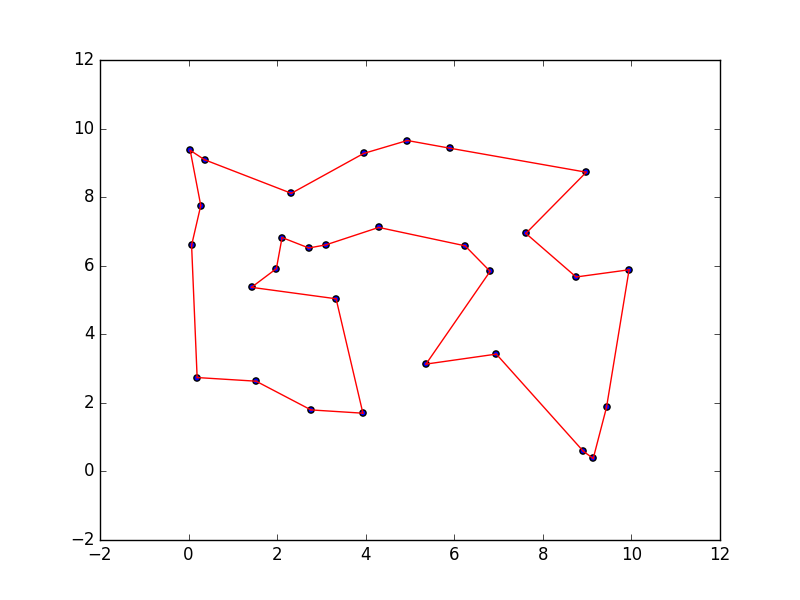
\includegraphics[width=0.5\textwidth]{img/tsp_solution_example.png}
\caption{Example of a solution to a TSP with 30 cities distributed uniformly at random. Each of the blue points represents a city. Each of the red lines indicates which city to travel to next. The solution shown is most likely optimal.}
\label{fig:tsp-example}
\end{figure}

The travelling salesman problem (TSP) is a classic mathematical problem well suited for the application of GAs. The premise of the TSP is as follows:

\begin{displayquote}
\textit{Given a list of cities and the distances between each pair of cities, what is the shortest possible route that visits each city exactly once and returns to the origin city?}
\end{displayquote}

The problem is renowned for being simple to grasp but computationally intensive to calculate an exact solution. The TSP has been shown to be NP-hard and a brute force solution requires O(n!) time. Algorithms with factorial time complexity become unworkable with anything other than very small datasets. GAs easily lend themselves to the travelling salesman problem. A GA makes no guarantees about finding an optimal solution to a TSP, but can be used to find an approximate solution in a reasonable amount of time given decent parameters. It is able to do this faster than with a basic brute force search because a GA will only examine a subset of solutions in the search space that may or may not include the optimum result, but should with good parameters converge towards the optimum solution.

\section{Program Description}
My solution to this assignment is implemented as a Python package with a basic command line interface. The installation of the package and the operation of the command line interface are described in detail in appendices \ref{appendix:installation} and \ref{appendix:cli} respectively.

The main implementation of the GA algorithm is within the sub-package \textit{tspsolver.ga}. This package contains a separate module for each of the components of the genetic algorithm. It also includes the simulator module, which is responsible for composing each of the components and running the genetic algorithm itself.

Each of the component modules contains an abstract base class for the particular type of component and several subclasses which provide concrete implementations of specific types of that component. For example, the crossover module contains a class \textit{AbstractCrossoverOperator} which implements operations common to all crossover operators and provides an abstract method \textit{\_crossover\_for\_chromosomes} which all subclasses must implement in order to derive the class. Provided that each of the components implement the specified interface, the \textit{Simulator} class will be able to setup and use the component without knowledge of the implementations details of the concrete component. In software engineering terms this architecture is known as the ``strategy'' design pattern. The strategy enables the behaviour of the algorithm to be dynamically selected at runtime. 

\begin{figure}[H]
\centering
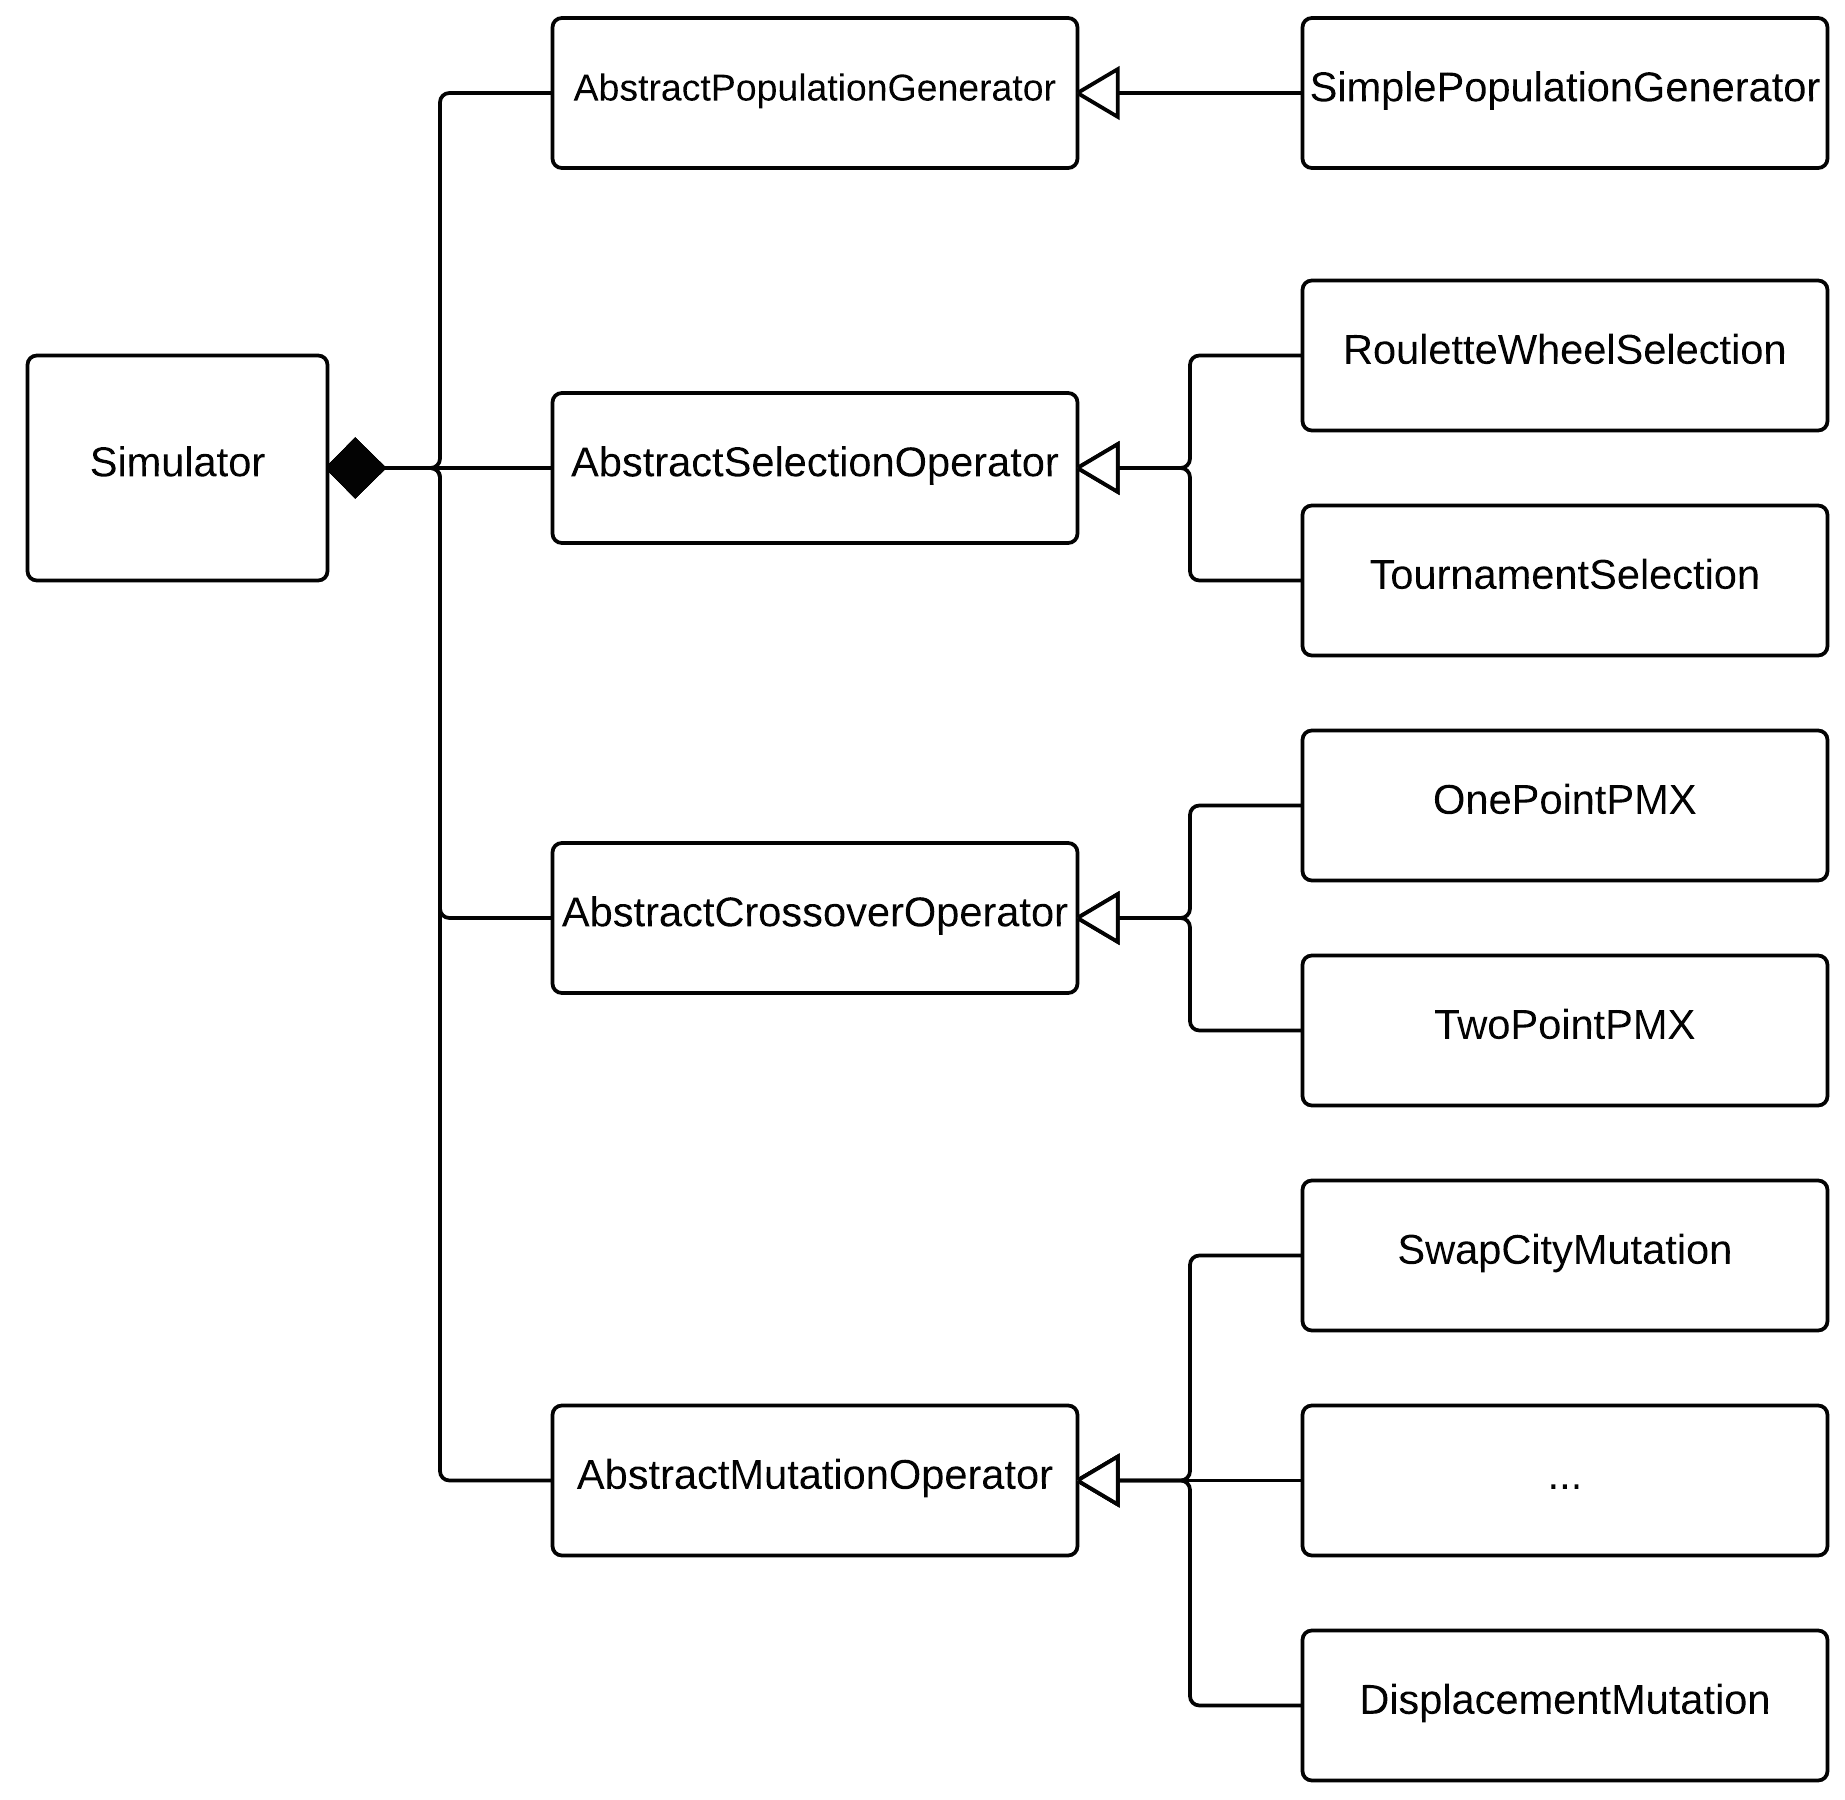
\includegraphics[width=0.5\textwidth]{img/class_diagram.png}
\caption{Class diagram for the simulator class and its components using the strategy pattern. The simulator is composed with one of each type of component. The abstract classes provide and common interface for the components. Concrete implementations of the components derive from the relevant base class}
\label{fig:class-diagram}
\end{figure}


My implementation takes this slightly further in that the \textit{Simulator} class which composes the components of the GA together actually dynamically loads the correct components using Python's reflection capabilities according to user supplied string parameters. The parameters for the application are supplied via a command line interface in the form of a JSON file. Information regarding the structure of the parameter file can be found in the appendix \ref{appendix:parameters}

Once instantiated the \textit{Simulator} takes a 2D matrix with two columns ($x$ and $y$ coordinates) and $n$ rows (equal to the number of cities) as a parameter to the evolve method. The evolve method runs converts the datasets into a distance matrix then approximates a solution using the genetic algorithm.

In addition to the main \textit{tspsolver.ga} sub-package there are four other modules. These are really just supporting code for the running the simulator and producing the analysis. These modules are:

\begin{itemize}
	\item \textbf{tsp\_generator} - Implements a small class for generating TSP datasets with uniformly random cities.
	\item \textbf{command} - Implements the command line interface for running the simulator and includes a couple of file loading and saving routines.
	\item \textbf{plotting} - Defines some custom plotting functions for producing the graphs used in this report.
	\item \textbf{tuning} - A basic class for using a grid search to automatically select GA parameters.
\end{itemize}

\section{Representation Discussion}
For my experiments I chose to use a path based representation for chromosomes. In a path based representation each chromosome is represented as an array of integers. The value of each integer element represents a single city in the dataset. In my program this integer corresponds to the $i^{th}$ row in the $2 \times n$ dataset. Each integer's position in the array indicates the order in which it will be visited. For example: in the array $[3, 4, 1, 5, 2]$ the first city to be visited would be city $3$. For city $3$ the tour then moves to city $4$ and from city $4$ to city $1$. 

Obviously since each city in the tour should only be visited once any valid solution should only contain a single occurrence of each city. Likewise because all cities must be visited exactly once each of cities in the dataset must be included in any valid solution. Therefore all valid solutions must be of size $n$ where $n$ is the number of cities in the dataset. In this representation format valid solutions are simply permutations of the enumeration of every city in the dataset.  

While many different representations of the TSP are possible \cite{larranaga1999genetic}, a path based representation remains the most natural. It is both intuitive for the beginner to understand (of which I am one personally) and has a large array of applicable genetic operators which can be utilised. Other approaches are possible as shown in ref. \cite{larranaga1999genetic}, but these are shown to either have poor results or have peculiarities in their representations. For example in a binary representation there are some seemingly valid encodings for which their are no valid cities.

However, this does not mean that a path based representation is without its downsides. The primary issues with encoding a set of cities as a chromosome for a TSP is ensuring that the genetic operators used will produce valid tours. As mentioned in the preceding paragraphs, a valid tour needs to be a permutation of the enumeration of all cities in the dataset. It is easy to see how traditional naive genetic operators would inevitably create invalid tours by producing a solution that visits the same city twice and excludes one or more cities.

\section{Algorithm Components \& Genetic Operators Discussion}
There are three main types of genetic operators that are typically used as part of a genetic algorithm. These are selection, crossover, and mutation. In my application I have implemented a variety of different genetic operators. Additionally I have used two different techniques for generating  of the initial populations. This section outlines the implementations I have used in the experiments in section \ref{sec:experiments} and provides a justification as to why they were chosen.

\subsection{Population Generation}
My genetic algorithm implementation has two different methods of initialising the population. The first type of population generation technique is purely random. The \textit{SimplePopulationGenerator} in the \textit{population\_generation} module simple create the desired population size by creating random permutations of the enumeration of the list of cities. 

Random initialisation is very general and works fine for all genetic operators tested in my application. However, it is painfully evident that some initial solutions are going to better than others. In an optimal solution a city will have the city will the shortest distance from it next in the chromosome sequence. In general, over a small local neighbourhood, a good heuristic might be to use the closest neighbours to a city as the adjacent neighbours in the chromosome ordered from closest to largest. 

This will not always yield great chromosome solutions. Contemplate the closest neighbours to a few points i \ref{fig:tsp-example} for a few moments and you will clearly see that the $k^{th}$ nearest element is not necessarily the $k{th}$ element in the optimal tour. However, especially for larger datasets, the cities in the immediate vicinity of one particular city are more likely to end up closer together in the chromosome.

With this intuition I created a second population generator \textit{KNNPopulationGenerator} which uses the $K$-nearest neighbours of a city to generate a chromosome. Specifically the algorithm works as follows: for each element of the population to be created it picks a city at random. An ordered list of the $K$-nearest neighbours to that city are then found where $K$ is equal to the total number of cities. The hope is that this is more likely to lead to initial chromosomes which have some portion of their chromosomes already in the correct place (or nearly in the correct place) than simply choosing at random. 

\subsection{Selection}
In genetic algorithm terms, selection is the method by which individuals from the current population are in order to produce a new population through crossover and mutation. A good selection technique should yield more ``good'' chromosomes for reproduction than bad ones. This is because the best solutions in the current population are generally more likely to produce even better offspring in the following generation. 

However, this does not mean that we should always just sort and take the best solutions because this rapidly leads to a lack of diversity. Consider a candidate TSP solution that yields a poor fitness because the just one of the connections geographically cuts from one side of the world to the other. In this scenario the fitness function ranks the solution as poor, but in reality it is quite close to being optimal! If a selection approach naively selects just the best looking solutions we are more likely to head towards local optima and potentially do not explore the full search space.

In my application, I have implemented two classic yet contrasting types of selection operator. The first selection procedure I implemented was \textit{Roulette Wheel} selection \cite{colin2002genetic}. Roulette wheel selection uses a probability distribution over each potential solution to be picked. Solutions are weighted proportionally to their fitness. \textit{Roulette Wheel} selection selects chromosomes are random and proportionally to their weighting. \textit{Roulette Wheel} selection gets its name from the fact that individuals are weighted in proportion to the area of a sector of a roulette wheel \cite{colin2002genetic}.

I chose to use \textit{Roulette Wheel} selection for two main reasons: firstly, it is very simple to implement and secondly, being one of the most basic techniques, it makes a nice yard stick which other techniques can be compared against. However, this approach has some well know downsides. \textit{Roulette Wheel} selection is well known to often be ``too random''. While candidate solutions are weighted such that more promising individuals are more likely to be picked there is still a huge amount of variation in which solutions actually get picked. This is especially true considering the shear number of solutions generated in even a moderately sized GA problem.

Because of the limitations of \textit{Roulette Wheel} selection I chose to also implement \textit{Tournament} selection \cite{colin2002genetic}. In \textit{Tournament} selection a subset of the total population of chromosomes is chosen at random. The chromosomes in this random subset are then compared against each other. In my implementation I have decided to make the simplest choice an implement \textit{strict} \textit{Tournament} selection where the chromosome with the biggest fitness is always the ``winner'' of the tournament. An alternative formulation is the use of \textit{soft} tournaments where the winner is probabilistically selected according to their fitness.

\textit{Tournament} selection is a very practical technique that is simple to implement, scales well, and can potentially be parallelised. Another key advantage over \textit{Roulette Wheel} selection is that \textit{Tournament} selection provides a parameter that directly adjusts the selection pressure applied by the selection operator. The selection pressure is the likelihood that an average individual will be selected over the fittest individual. Changing the size of the tournament influences how likely it is that weaker chromosomes will survive the selection process. Bigger tournaments lead to an increase chance of a better individual entering the tournament; therefore increasing the probability that they'll be selected and visa versa. However, it is also worth noting that \textit{Tournament} selection still suffers from the same issues as \textit{Roulette Wheel} selection. The random nature of the algorithm can mean that the distribution you get is skewed and not fully representative.

\subsection{Crossover}
The crossover operator is used to recombine selected individuals to form a new population with solutions that are different (and hopefully better) than the previous population. A good crossover operator should attempt to preserve the best portions of the selected chromosomes. Without the counter effect of a mutation operator a good crossover operator should eventually cause the GA to converge to a (possibly not optimal) solution.

The implementations of the crossover operators that I have used in my application can be found in the \textit{crossover} module. I have implemented three different crossover operators, two of which are fairly similar to one another.

The first two operators I have implemented are \textit{OnePointPMX} and \textit{TwoPointPMX}. As their name suggests the only different in their implementation is the number of pivot points used to define which parts of the chromosomes get recombined (similar to regular one and two point crossover). PMX crossover begins by copying some sub section of the parent chromosome to the child.



\subsection{Mutation}

\section{Experiments Performed}
\label{sec:experiments}

\section{Discussion and Analysis}
\section{Conclusions and Future Work}


% needed in second column of first page if using \IEEEpubid
%\IEEEpubidadjcol

% An example of a floating figure using the graphicx package.
% Note that \label must occur AFTER (or within) \caption.
% For figures, \caption should occur after the \includegraphics.
% Note that IEEEtran v1.7 and later has special internal code that
% is designed to preserve the operation of \label within \caption
% even when the captionsoff option is in effect. However, because
% of issues like this, it may be the safest practice to put all your
% \label just after \caption rather than within \caption{}.
%
% Reminder: the "draftcls" or "draftclsnofoot", not "draft", class
% option should be used if it is desired that the figures are to be
% displayed while in draft mode.
%
%\begin{figure}[!t]
%\centering
%\includegraphics[width=2.5in]{myfigure}
% where an .eps filename suffix will be assumed under latex, 
% and a .pdf suffix will be assumed for pdflatex; or what has been declared
% via \DeclareGraphicsExtensions.
%\caption{Simulation Results}
%\label{fig_sim}
%\end{figure}

% Note that IEEE typically puts floats only at the top, even when this
% results in a large percentage of a column being occupied by floats.


% An example of a double column floating figure using two subfigures.
% (The subfig.sty package must be loaded for this to work.)
% The subfigure \label commands are set within each subfloat command, the
% \label for the overall figure must come after \caption.
% \hfil must be used as a separator to get equal spacing.
% The subfigure.sty package works much the same way, except \subfigure is
% used instead of \subfloat.
%
%\begin{figure*}[!t]
%\centerline{\subfloat[Case I]\includegraphics[width=2.5in]{subfigcase1}%
%\label{fig_first_case}}
%\hfil
%\subfloat[Case II]{\includegraphics[width=2.5in]{subfigcase2}%
%\label{fig_second_case}}}
%\caption{Simulation results}
%\label{fig_sim}
%\end{figure*}
%
% Note that often IEEE papers with subfigures do not employ subfigure
% captions (using the optional argument to \subfloat), but instead will
% reference/describe all of them (a), (b), etc., within the main caption.


% An example of a floating table. Note that, for IEEE style tables, the 
% \caption command should come BEFORE the table. Table text will default to
% \footnotesize as IEEE normally uses this smaller font for tables.
% The \label must come after \caption as always.
%
%\begin{table}[!t]
%% increase table row spacing, adjust to taste
%\renewcommand{\arraystretch}{1.3}
% if using array.sty, it might be a good idea to tweak the value of
% \extrarowheight as needed to properly center the text within the cells
%\caption{An Example of a Table}
%\label{table_example}
%\centering
%% Some packages, such as MDW tools, offer better commands for making tables
%% than the plain LaTeX2e tabular which is used here.
%\begin{tabular}{|c||c|}
%\hline
%One & Two\\
%\hline
%Three & Four\\
%\hline
%\end{tabular}
%\end{table}


% Note that IEEE does not put floats in the very first column - or typically
% anywhere on the first page for that matter. Also, in-text middle ("here")
% positioning is not used. Most IEEE journals use top floats exclusively.
% Note that, LaTeX2e, unlike IEEE journals, places footnotes above bottom
% floats. This can be corrected via the \fnbelowfloat command of the
% stfloats package.







% if have a single appendix:
%\appendix[Proof of the Zonklar Equations]
% or
%\appendix  % for no appendix heading
% do not use \section anymore after \appendix, only \section*
% is possibly needed

% use appendices with more than one appendix
% then use \section to start each appendix
% you must declare a \section before using any
% \subsection or using \label (\appendices by itself
% starts a section numbered zero.)
%


\appendices

\section{Installation of Program}
\label{appendix:installation}

\section{Command Line Interface}
\label{appendix:cli}
This appendix provides an overview of the operation of the CLI for the application.

\section{Parameters}
\label{appendix:parameters}
%Some text for the appendix.

% use section* for acknowledgement
%\section*{Acknowledgment}
%
%
%The authors would like to thank...


% Can use something like this to put references on a page
% by themselves when using endfloat and the captionsoff option.
\ifCLASSOPTIONcaptionsoff
  \newpage
\fi



% trigger a \newpage just before the given reference
% number - used to balance the columns on the last page
% adjust value as needed - may need to be readjusted if
% the document is modified later
%\IEEEtriggeratref{8}
% The "triggered" command can be changed if desired:
%\IEEEtriggercmd{\enlargethispage{-5in}}

% references section

% can use a bibliography generated by BibTeX as a .bbl file
% BibTeX documentation can be easily obtained at:
% http://www.ctan.org/tex-archive/biblio/bibtex/contrib/doc/
% The IEEEtran BibTeX style support page is at:
% http://www.michaelshell.org/tex/ieeetran/bibtex/
%\bibliographystyle{IEEEtran}
% argument is your BibTeX string definitions and bibliography database(s)
%\bibliography{IEEEabrv,../bib/paper}
%
% <OR> manually copy in the resultant .bbl file
% set second argument of \begin to the number of references
% (used to reserve space for the reference number labels box)
\bibliographystyle{plain}
\bibliography{references}
%\begin{thebibliography}{1}
%
%\bibitem{IEEEhowto:kopka}
%H.~Kopka and P.~W. Daly, \emph{A Guide to \LaTeX}, 3rd~ed.\hskip 1em plus
%  0.5em minus 0.4em\relax Harlow, England: Addison-Wesley, 1999.
%
%\end{thebibliography}

% biography section
% 
% If you have an EPS/PDF photo (graphicx package needed) extra braces are
% needed around the contents of the optional argument to biography to prevent
% the LaTeX parser from getting confused when it sees the complicated
% \includegraphics command within an optional argument. (You could create
% your own custom macro containing the \includegraphics command to make things
% simpler here.)
%\begin{biography}[{\includegraphics[width=1in,height=1.25in,clip,keepaspectratio]{mshell}}]{Michael Shell}
% or if you just want to reserve a space for a photo:

%\begin{IEEEbiography}[{\includegraphics[width=1in,height=1.25in,clip,keepaspectratio]{picture}}]{John Doe}
%\blindtext
%\end{IEEEbiography}

% You can push biographies down or up by placing
% a \vfill before or after them. The appropriate
% use of \vfill depends on what kind of text is
% on the last page and whether or not the columns
% are being equalized.

%\vfill

% Can be used to pull up biographies so that the bottom of the last one
% is flush with the other column.
%\enlargethispage{-5in}



% that's all folks
\end{document}


